\subsection{Separating vertex initialization from the update rule}
The preceding AC-FW comparison changes both initialization and the
subsequent rule. We therefore run a controlled $2\times2$ study on the
same 70 instances: the original point or the compulsory LMO vertex,
combined with AC updates or ordinary backtracking (BT). All four cells
pay for two function values, two gradients, and two LMOs at the two
preprocessing points. They retain both scalar lower bounds and the same
secant curvature. BT's stored initial estimate is twice the AC estimate,
so its first halving gives exactly the same first trial. Afterwards BT
halves and doubles its estimate, while AC uses the fixed damping above.
AC/vertex is the native comparator; the other three cells are controls,
not the published AC-FW algorithm. No curvature or reference quantities
are supplied to their step rules.

There are 280 runs with the previous outer cap and tolerance. All 70
AC/vertex runs match the earlier native comparator's objective,
certificate, and oracle counts exactly; no new independent instances
are added. Table~\ref{tab:factorial} uses separate budgets for function
and gradient calls. Each value is the last fully available certificate
before that oracle budget, reconstructed from the complete trace before
sampling. It is not an interpolation between saved trace rows. Other
oracle types are unrestricted. All nonterminal runs can reach 1000
function calls before hitting the outer cap, so this primary budget
comparison is not censored by that cap.

On the active family, moving to the LMO vertex changes the number of
certified runs at 1000 function calls from 1 to 10 for AC and from 0 to
10 for BT. Thus the earlier 10/10 versus 0--1/10 comparison did not
isolate the subsequent curvature update. The median paired certificate
ratio BT/AC from the vertex is 1.049, with descriptive percentile-bootstrap
interval $[0.935,1.257]$. Vertex/original ratios are 0.0351 for AC and
0.0150 for BT. These describe the ten matched instances at a fixed
budget, not speedup factors or a population-level ranking; completed
runs stop near the tolerance. All 84 comparisons, including other
oracle budgets and families, are recorded with 10000 bootstrap resamples
and seed 20261015, without a multiple-comparison correction.

On Bike Sharing at 1000 function calls, AC certifies 6/10 starts from the
original point and 7/10 from the vertex; BT certifies 2/10 and 5/10.
At 1000 gradients BT/original certifies 6/10, like AC/original. The oracle
unit changes the comparison. The scaled active family remains unsolved
by all four cells within the reported budgets. Figure~\ref{fig:initialization}
shows the function-budget profiles.

\begin{table}[htbp]
\centering\small
\caption{Controlled starting-point/update-rule ablation. Each cell has the same preprocessing cost and first trial curvature. Successes and median certificates at separate budgets of 1000 function or gradient calls, over ten seeds. Other oracle types are unrestricted; the outer cap remains 1000.}
\label{tab:factorial}
\begin{tabular}{llrrrr}
\hline
 & & \multicolumn{2}{c}{1000 function calls} & \multicolumn{2}{c}{1000 gradient calls} \\
Rule & Start & Successes & Median $U$ & Successes & Median $U$ \\
\hline
\multicolumn{6}{l}{\textbf{active}} \\
AC & original & 1/10 & 2.06e-04 & 1/10 & 2.06e-04 \\
AC & vertex & 10/10 & 7.93e-06 & 10/10 & 7.93e-06 \\
BT & original & 0/10 & 5.18e-04 & 0/10 & 2.61e-04 \\
BT & vertex & 10/10 & 8.44e-06 & 10/10 & 8.44e-06 \\
\hline
\multicolumn{6}{l}{\textbf{active\_scaled}} \\
AC & original & 0/10 & 2.00e-03 & 0/10 & 2.00e-03 \\
AC & vertex & 0/10 & 2.68e-03 & 0/10 & 2.68e-03 \\
BT & original & 0/10 & 3.72e-03 & 0/10 & 1.86e-03 \\
BT & vertex & 0/10 & 3.60e-03 & 0/10 & 1.84e-03 \\
\hline
\multicolumn{6}{l}{\textbf{bike\_poisson}} \\
AC & original & 6/10 & 9.72e-06 & 6/10 & 9.72e-06 \\
AC & vertex & 7/10 & 9.53e-06 & 7/10 & 9.53e-06 \\
BT & original & 2/10 & 6.72e-05 & 6/10 & 9.94e-06 \\
BT & vertex & 5/10 & 2.20e-05 & 5/10 & 1.11e-05 \\
\hline
\end{tabular}
\end{table}


\paragraph{A geometric explanation on the planted instances.}
Let $w=\operatorname{sign}(x^*)$, zero off its support, and
$\sigma(x)=R-w^\top x\ge0$. The optimal face is
$F=\{x\in Q:\sigma(x)=0\}$. Every FW update satisfies exactly
\[
 \sigma(x+\alpha(s-x))=(1-\alpha)\sigma(x)+\alpha\sigma(s).
\]
If selected vertices lie in $F$ and all steps are strictly below 1,
a point outside $F$ retains positive slack at every finite iteration.
A full initial move to a vertex in $F$ removes this slack immediately.
For the planted normal $v$, $|v_i|\le0.6$ off the support, so
\[
 f(x)\ge\lambda(R-v^\top x)\ge0.4\lambda\sigma(x).
\]
The last inequality uses $\|x_{\rm off}\|_1\le\sigma(x)$.
This is an application of the familiar face geometry of vanilla
FW~\cite{braun}, not a new acceleration mechanism.

Post-run diagnostics replay all 120 controls in the three active families,
using the planted support only after solving. The slack identity and
lower bound hold throughout. On the active family the initial LMO vertex
lies in $F$ for all ten seeds, and both vertex-start cells stay in $F$.
BT/original takes no full step and retains positive final slack in all
ten runs; AC/original takes one full step in its sole successful run.
At the outer cap, BT/original's smallest final slack among these ten
runs is about $9.98\cdot10^{-4}$. Since $\lambda=0.15$, the lower
bound above already exceeds the target $10^{-5}$ in every run;
failure here is not merely a loose stopping certificate.
In the high-dimensional family the initial vertex is in $F$ for eight
seeds, and the corresponding vertex-start runs stay there. In the scaled
family only one initial vertex is in $F$, and no vertex-start run remains
in $F$ throughout. This explains the observed initialization sensitivity
on these constructed examples without a claim for general applications.

\begin{figure}[htbp]
\centering
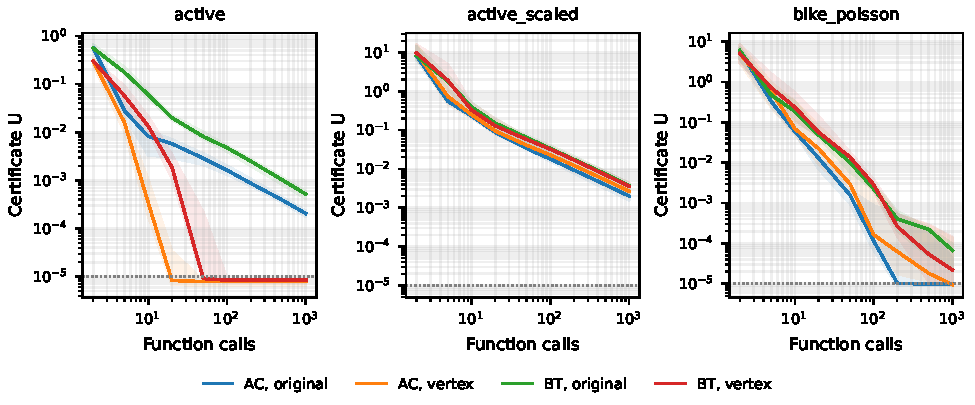
\includegraphics[width=\textwidth]{figures/initialization_effect.pdf}
\caption{Controlled ablation: median certificate and interquartile band
at the displayed function-call budgets. Every prefix includes common
preprocessing. Runs stop at $U\le10^{-5}$ or 1000 outer trials; completed
certificates are carried forward. The displayed function budgets are
reached before the outer cap in nonterminal runs. Lines between displayed
budgets are for visualization; the CSV contains the actual prefix values.}
\label{fig:initialization}
\end{figure}
